\documentclass[titlepage,a4paper,12pt]{report}
\usepackage{amssymb,amsfonts,amsmath}
\usepackage{tikz}
\usetikzlibrary{arrows}
\newcommand\Interval[4]{%
  \begin{tikzpicture}[text height=1ex]%
    \draw[<-] (0,0) -- (1,0);
    \draw[{#3-#4}] (1,0) node[label=below:{#1}] {} -- (2,0) node[label=below:{#2}] {};
    \draw[->] (2,0) -- (3,0);
  \end{tikzpicture}
}
%\usepackage{fullpage}
\usepackage{graphicx}
%\usepackage[cc]{titlepic}
\usepackage{amsthm}
\newtheorem{definition}{Definition}[section]
\newtheorem{example}{Example}[section]
\newtheorem{theorem}{Theorem}[section]
\newtheorem{exercise}{Exercise}[section]
\newtheorem{corollary}{Corollary}[section]
\newtheorem{proposition}{Proposition}[section]
\pdfpagewidth 8.5in
\pdfpageheight 11in
\setlength\topmargin{-0.5in}
\setlength\headheight{0in}
\setlength\headsep{0in}
\setlength\textheight{9.5in}
\setlength\textwidth{7.0in}
\setlength\oddsidemargin{-0.5in}
\setlength\evensidemargin{1.0in}
\setlength\parindent{0.25in}
\setlength\parskip{0.25in}
%\begin{titlepage}
%\usepackage{titlepic}
%\titlepic{
\includegraphics[width=0.2\textwidth]{uz1.png}}
%
%\title{\textbf{HMTH111 Calculus 2}}
%\author{Nhawu. G\\
%		Department of Mathematics\\
%		University of Zimbabwe, ZIM}
%
%\end{titlepage}

\begin{document}
\begin{titlepage}
 
\begin{center}
 
 
% Upper part of the page

\includegraphics[width=0.15\textwidth]{uz1.png}\\[1cm]
 
\textsc{\LARGE University of Zimbabwe}\\[1.5cm]
 
\textsc{\Large HMTH101 CALCULUS 1}\\[0.5cm]
 
 
% Title

{ \huge \bfseries Calculus of Single Variables}\\[0.4cm]
 

 
% Author and supervisor
\begin{minipage}{0.4\textwidth}
\begin{center} \large
\emph{Author:}\\
G. \textsc{Nhawu}
\end{center}
\end{minipage}
\begin{minipage}{0.4\textwidth}
\begin{flushright} \large
\emph{Department:} \\
\textsc{Mathematics}
\end{flushright}
\end{minipage}

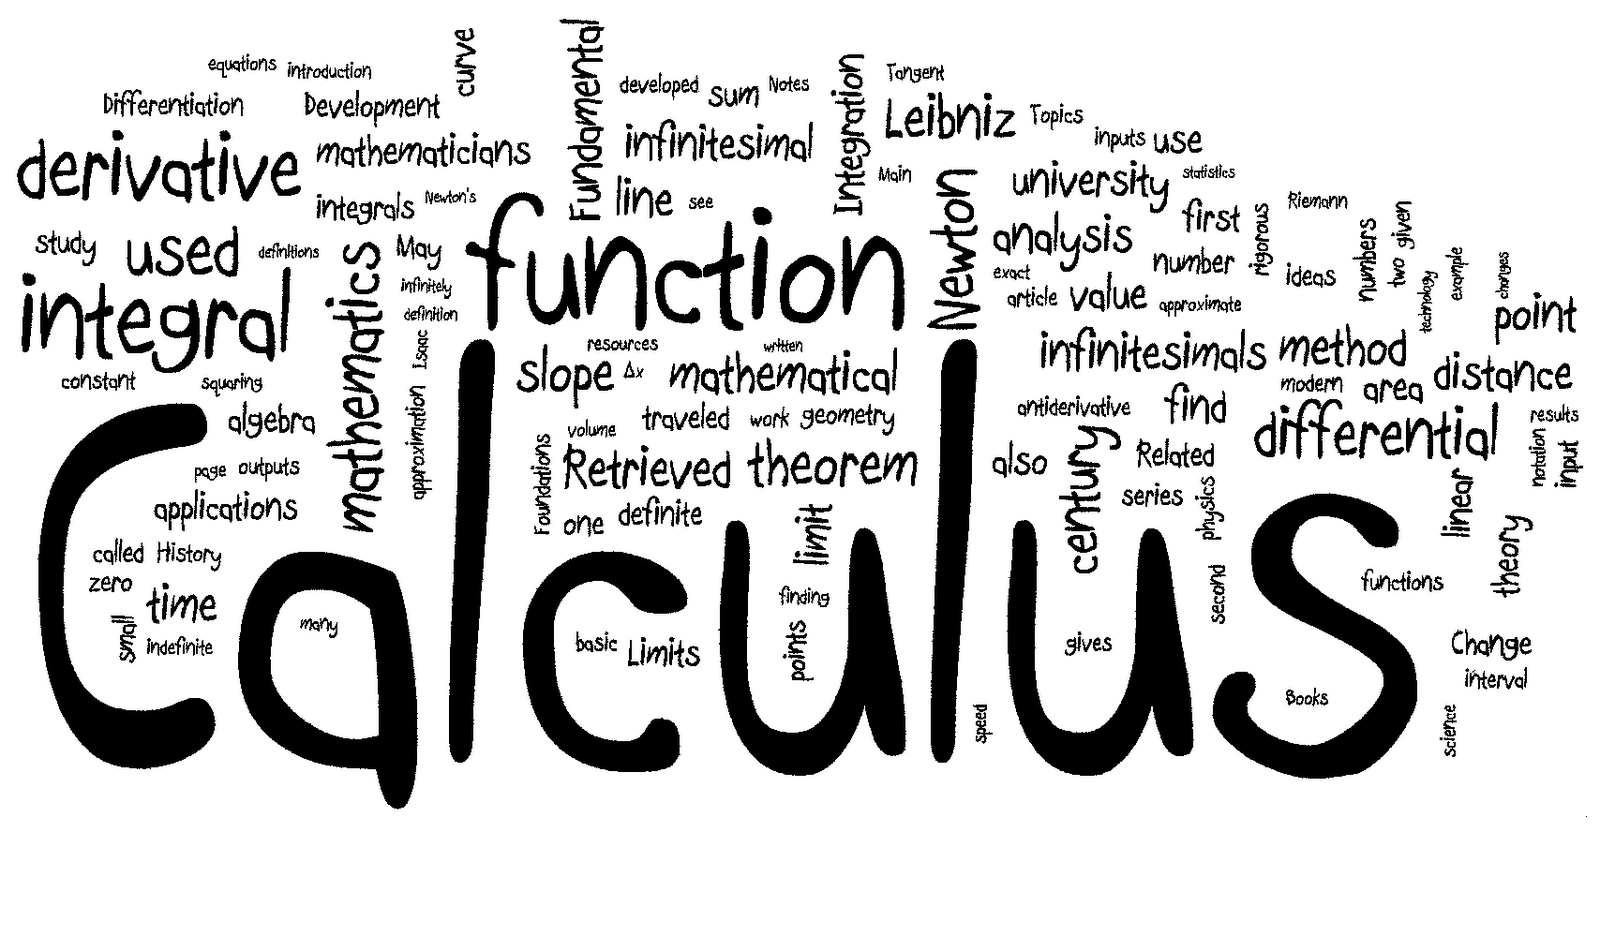
\includegraphics[width=0.98\textwidth]{calculus2.png}\\[1cm]
 \vfill
 
 
% Bottom of the page
{\large \today}
 
\end{center}
 
\end{titlepage}

\tableofcontents
\begin{abstract}
\begin{center}
	\small{\parbox{20cm}{
		\begin{raggedright}
		{\small
		\textit{Everybody is a genius. But if you judge a fish by its ability to climb a tree, it will live its whole life believing that it is stupid.}
 }
 
				\vspace{.5cm}\hfill{---Albert Einstein}
		\end{raggedright}
	}
} 
\end{center}
Calculus is one of the milestones of Western thought. Building on ideas of
Archimedes, Fermat, Newton, Leibniz, Cauchy, and many others, the calculus is
arguably the cornerstone of modern science. Any well-educated person should
at least be acquainted with the ideas of calculus, and a scientifically literate person
must know calculus solidly. Calculus has two main aspects: differential calculus and integral calculus.
Differential calculus concerns itself with rates of change. Various types of change,
both mathematical and physical, are described by a mathematical quantity called
the derivative. Integral calculus is concerned with a generalized type of addition,
or amalgamation, of quantities. Many kinds of summation, both mathematical and
physical, are described by a mathematical quantity called the integral.

\noindent Calculus is one of the most important parts of mathematics. It is fundamental to all
of modern science. How could one part of mathematics be of such central importance?
It is because calculus gives us the tools to study rates of change and motion.
All analytical subjects, from biology to physics to chemistry to engineering to mathematics,
involve studying quantities that are growing or shrinking or moving, in
other words, they are changing. Astronomers study the motions of the planets,
chemists study the interaction of substances, physicists study the interactions of
physical objects. All of these involve change and motion.
\footnote{To Archimedes, Pierre de Fermat, Isaac Newton, and Gottfried Wilhelm
von Leibniz, the fathers of calculus}
\footnote{The true sign of intelligence is not knowledge but imagination------
Albert Einstein }
\end{abstract}
\chapter{The Basics}
\begin{center}
	\small{\parbox{20cm}{
		\begin{raggedright}
		{\small
		\textit{Learning never exhausts the mind.}
 }
 
				\vspace{.5cm}\hfill{---Leonardo da Vinci}
		\end{raggedright}
	}
} 
\end{center}
\section{Number Systems}
Mathematics has its own language with numbers as the alphabet. The language is given structure
with the aid of connective symbols, rules of operation, and a rigorous mode of thought (logic). The number systems that we use in calculus are the \textit{natural numbers}, the \textit{integers}, the \textit{rational numbers}, and the \textit{real numbers}. Let us describe each of these :
\begin{enumerate}
\item  The \textbf{natural numbers} are the system of positive counting numbers $1,2,3\dots .$ We denote the set of all natural numbers by $\mathbb{N}$.
\[\mathbb{N}=\{1,2,3,4,5,6,7,8,\dots\}.\]
\item The \textbf{integers} are the positive and negative whole numbers and zero, $\dots ,-3,-2,-1,0,1,2,3,\dots .$ We denote the set of all integers by $\mathbb{Z}$.
\[\mathbb{Z}=\{\dots, -4,-3,-2,-1,0,1,2,3,4,\dots\}.\]
\item The \textbf{rational numbers} are quotients of integers or \textbf{fractions}, such as $\frac{2}{3}, -\frac{5}{4}$. Any number of the form $\dfrac{p}{q}$, with $p,q \in \mathbb{Z}$ and $q\neq 0$, is a rational number. We denote the set of all rational numbers by $\mathbb{Q}$.
\[\mathbb{Q}=\left\{\dfrac{p}{q}\biggl|p,q\in \mathbb{Z}, q\neq 0\right\}.\]
\item The \textbf{real numbers} are the set of all decimals, both terminating and non-terminating. We denote the set of all real numbers by $\mathbb{R}$. A decimal number of the form $x=3.16792$ is actually a rational number, for it represents 
\begin{equation*}
x=3.16792=\dfrac{316792}{100000}.
\end{equation*}
A decimal number of the form 
\begin{equation*}
m=4.27519191919\dots ,
\end{equation*}
with a group of digits that repeats itself interminably, is also a rational number.
To see this, notice that 
\begin{equation*}
100\cdot m=427.519191919\dots 
\end{equation*}  
and therefore we may subtract
\begin{eqnarray*}
100m=427.519191919\dots \\
m=4.27519191919\dots
\end{eqnarray*}
Subtracting, we see that 
\begin{equation*}
99m=423.244
\end{equation*}
or 
\begin{equation*}
m=\dfrac{423244}{99000}.
\end{equation*}
So, as we asserted, $m$ is a rational number  or quotient of integers. To  indicate recurring decimals we sometimes place dots over the repeating cycle of digits, e.g., $m=4.275\dot{1}\dot{9},\\ \frac{19}{6}=3.1\dot{6}$.

Another kind of decimal number is one which has a non-terminating decimal expansion \textit{that does not keep repeating}. An example is $\pi=3.14159265\dots $. Such a number is \textit{irrational}, that is, it \textit{cannot} be expressed as the quotient of two integers. 

In summary : There are three types of real numbers : (i)\, terminating decimals, \quad (ii)\, non-terminating decimals that repeat, \quad (iii)\, non-terminating decimals that do not repeat. Types (i) and (ii) are rational numbers. Type (iii) are irrational numbers.
 
The geometric representation of real numbers as points on a line is called the \textit{real axis}. Between any two rational numbers on the line there are infinitely many rational numbers. This leads us to call the set of rational numbers an \textit{everywhere dense set}.

Real numbers are characterised by three fundamental \textit{properties} :\\
\begin{enumerate}
\item \textbf{algebraic} means formalisations of the rules of calculation (addition, subtraction, multiplication, division). Example : $2(3+5)=2\cdot3 +2\cdot 5=6+10=16 $.
\item \textbf{order} denote inequalities. Example : $-\dfrac{3}{4}<\dfrac{1}{3}$.
\item \textbf{completeness} implies that there are ``no gaps'' on the real line.
\end{enumerate}
\textbf{Algebraic properties} of the reals for \textit{addition} ($a,b,c\in \mathbb{R}$) are :
\begin{itemize}
\item[(A1)] $a+(b+c)=(a+b)+c$. \textit{associativity}
\item[(A2)] $a+b=b+a$. \textit{commutativity}
\item[(A3)] There is a $0$ such that $a+0=a$.\quad  \textit{identity}
\item[(A4)] There is an $x$ such that $a+x=0$. \quad \textit{inverse}
\end{itemize}
Why these rules? They define an \textit{algebraic structure} (commutative group). Now define analogous algebraic properties for \textit{multiplication} :
\begin{itemize}
\item[(M1)] $a(bc)=(ab)c$.
\item[(M2)] $ab=ba$.
\item[(M3)] There is a $1$ such that $a\cdot 1=a$.
\item[(M4)] There is an $x$ such that $ax=1$ for $a\neq 0$.
\end{itemize}
Finally, connect \textit{multiplication} and \textit{addition} :
\begin{itemize}
\item[(D)] $a(b+c)=ab+ac$. \textit{distributivity}
\end{itemize}
These $9$ rules define an algebraic structure called a \textit{field}.

\textbf{Order properties} of the reals are :
\begin{itemize}
\item[(O1)] for any $a,b\in \mathbb{R}, \, a\leq b$ or $b\leq a$. \textit{totality of ordering I}
\item[(O2)] if $a\leq b$ and $b\leq a$, then $a=b$. \textit{totality of ordering II}
\item[(O3)] if $a\leq b$ and $b\leq c$, then $a\leq c$. \textit{transitivity}
\item[(O4)] if $a\leq b$, then $a+c\leq b+c$. \textit{order under addition}
\item[(O5)] if $a\leq b$ and $c\geq 0$, then $ac\leq bc$. \textit{order under multiplication} 
\end{itemize}
Some useful rules for calculations with inequalities are : If $a,b,c$ are real numbers, then :
\begin{enumerate}
\item if $a<b$ and $c<0 \Rightarrow bc<ac$.
\item if $a<b \Rightarrow -b<-a$.
\item if $a>0\Rightarrow \dfrac{1}{a}>0$.
\item if $a$ and $b$ are both positive or negative, then $a<b\Rightarrow \dfrac{1}{b} <\dfrac{1}{a}$.
\end{enumerate}
The \textbf{completeness property} can be understood by the following construction of the real numbers :
Start with the counting numbers $1,2,3,\dots .$
\begin{itemize}
\item $\mathbb{N}=\{1,2,3,4,\dots \}$ natural numbers $\Rightarrow$ Can we solve $a+x=b$ for $x$?
\item $\mathbb{Z}=\{\dots , -2,-1,0,1,2,\dots\}$ integers $\Rightarrow$ Can we solve  $ax=b$ for $x$?
\item $\mathbb{Q} =\{\frac{p}{q} | p,q \in \mathbb{Z}, q\neq 0\}$ rational numbers $\Rightarrow$ Can we solve $x^2=2$ for $x$?
\item $\mathbb{R}$ real numbers, for example : The positive solution to the equation $x^2=2$ is $\sqrt{2}$. This is an irrational number whose decimal representation is not eventually repeating.
\end{itemize}

\begin{equation*}
\Rightarrow \boxed {\mathbb{N}\subset \mathbb{Z}\subset \mathbb{Q}\subset \mathbb{R}}
\end{equation*}
In summary, the real numbers $\mathbb{R}$ are \textit{complete} in the sense that they correspond to all points on the real line, i.e., there are no ``holes'' or ``gaps'', whereas the rationals have ``holes'' (namely the irrationals).

\textbf{You Try It :} What type of real number is $3.41287548754875\dots$? Can you express this number in more compact form?
\end{enumerate}
\section{Intervals}
\begin{definition}
A subset of the real line is called an interval if it contains at least two numbers and all the real numbers between any of its elements.
\end{definition}
\textbf{Examples :} 
\begin{enumerate}
\item $x>-2$ defines an \textit{infinite interval}. Geometrically, it corresponds to a \textit{ray} on the real line.
\item $3\leq x\leq 6$ defines a \textit{finite interval}. Geometrically, it corresponds to a \textit{line segment} on the real line.
\end{enumerate}
\textbf{Finite Intervals.} Let $a$ and $b$ be two points such that $a<b$. By the \textit{open interval} $(a,b)$ we mean the set of all points between $a$ and $b$, that is, the set of all $x$ such that $a<x<b$. By the \textit{closed interval} $[a,b]$ we mean the set of all points between $a$ and $b$ or equal to $a$ or $b$, that is, the set of all $x$ such that $a\leq x\leq b$. The points $a$ and $b$ are called the \textit{endpoints} of the intervals $(a,b)$ and $[a,b]$.
\begin{center}
 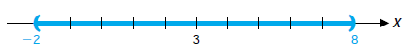
\includegraphics[width=0.4\textwidth]{open.png}\\[1cm]
  \end{center}
\noindent By a \textit{half-open interval} we mean an open interval $(a,b)$ together with one of its endpoints. There are two such intervals : $[a,b)$ is the set of all $x$ such that $a\leq x<b$ and $(a,b]$ is the set of all $x$ such that $a<x\leq b$.

\noindent \textbf{Infinite Intervals.} Let $a$ be any number. The set of all points $x$ such that $a<x$ is denoted by $(a,\infty)$, the set of all points $x$ such that $a\leq x$ is denoted by $[a,\infty)$. Similarly, $(-\infty ,b )$ denotes the set of all points $x$ such that $x<b$ and $(-\infty ,b]$ denotes the set of all $x$ such that $x\leq b$.
\begin{center}
 
\includegraphics[width=0.4\textwidth]{infinite.png}\\[1cm]
  \end{center}
\section{Solving Inequalities}
Solve inequalities to find intervals of $x\in \mathbb{R}$. Set of all solutions is the \textit{solution set} of the inequality.
\textbf{Examples:}
\begin{enumerate}
\item \begin{eqnarray*}
2x-1 &<& x+3 \\
2x &<& x+4\\
x &<& 4.
\end{eqnarray*}
\item For what values of $x$ is $x+3(2-x)\geq 4-x$?
\begin{eqnarray*}
x+3(2-x) &\geq &  4-x \quad \hbox{when} \\
x+6-3x &\geq &  4-x\\
6-2x &\geq &  4-x\\
2 &\geq & x \Rightarrow x\leq 2.
\end{eqnarray*}
\item For what values of $x$ is $(x-4)(x+3)<0$?

\noindent \textbf{Case 1:}  \quad  $(x-4)>0$ \quad \hbox{and} \quad $(x+3)<0, \Longrightarrow x>4$ \quad \hbox{and}\quad $x<-3$. \\
\noindent \textbf{Impossible} \quad \hbox{since $x$ cannot be both greater than $4$ and less than $-3$}.\\
\noindent \textbf{Case 2:}  \quad $(x-4)<0$ \quad \hbox{and} \quad $(x+3)>0, \Longrightarrow x<4$ \quad \hbox{and} \quad $x>-3\Longrightarrow -3<x<4$.

\end{enumerate}
\textbf{You Try It:} Solve the inequality $\dfrac{2}{x-1}<\dfrac{3}{2x+1}$.
\section{The Absolute Value}
It is a quantity that gives the \textit{magnitude} or \textit{size} of a real number. The \textbf{absolute value} or \textbf{modulus} of a real number $x$, denoted by $|x|$, is given by 
\[|x| = \left\{ 
\begin{array}{l l}
  x, & \quad \hbox{if}~~~ x\geq 0 \\
 -x, & \quad \hbox{if}~~~ x<0.\\ \end{array} \right. \]
 Geometrically, $|x|$ is the distance between $x$ and $0$.  For example, $|-6|=6, \, |5|=5, \, |0|=0$.
 \begin{center}
 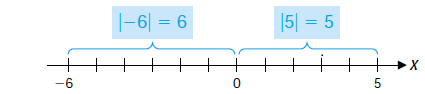
\includegraphics[width=0.4\textwidth]{absolute.png}\\[1cm]
  \end{center}
 \subsection{Properties of the Absolute Value }
 \begin{enumerate}
 \item The absolute value of a real number $x$ is non-negative, that is, $|x|\geq 0$.
 \item The absolute value of a real number $x$ is zero if and only if $x=0$, that is, $|x|=0\Longleftrightarrow x=0$.
 \item In general, if $x$ and $y$ are any two numbers, then 
 \begin{enumerate}
 \item $-|x|\leq x\leq |x|$.
 \item $|-x|=|x|$ and $|x-y|=|y-x|$.
 \item $|x|=|y|$ implies $x=\pm y$.
 \item $|xy|=|x|\cdot |y|$ and $\left|\dfrac{x}{y}\right|=\dfrac{|x|}{|y|}$ if $y\neq 0$.
 \item $|x+y|\leq |x|+|y|$. (Triangle inequality)
 \end{enumerate}
 \item If $a$ is any positive number, then 
 \begin{enumerate}
 \item $|x|=a$ if and only if $x=\pm a$.
 \item $|x|<a$ if and only if $-a<x<a$.
 \item $|x|>a$ if and only if $x>a$ or $x<-a$.
 \item $|x|\leq a$ if and only if $-a\leq x\leq a$.
 \item $|x|\geq a$ if and only if $x\geq a$ or $x\leq -a$.
 \end{enumerate}
 \end{enumerate}
 \textbf{Example:} Show that for all real numbers $x$, $|-x|=|x|$.\\
 \textbf{Solution:} If $x\in \mathbb{R}$, then either $x>0, x=0$ or $x<0$. If $x>0$, then $-x<0$. Thus, $|-x|=-(-x)=x=|x|$, that is, $|-x|=|x|$. \\
If $x=0$, then $|-x|=|-0|=|0|=0$, that is, $|-x|=|x|$.\\
If $x<0$, then $-x>0$. Now $|x|=-x=|-x|$ since $-x>0$.\\
Therefore in all cases $|-x|=|x|$.

\noindent \textbf{Solving an Equation with Absolute Values:} Solve the equation $|2x-3|=7$.

\noindent \textbf{Solution:} Hence $2x-3=\pm 7$, so there are two possibilities, 
\begin{eqnarray*}
2x-3 &=& 7 \quad  \quad 2x-3 =-7\\
2x &=& 10 \quad \quad 2x = -4\\
x &=& 5 \quad \quad x = -2
\end{eqnarray*}
The solutions of $|2x-3|=7$ are $x=5$ and $x=-2$.

\noindent \textbf{Solving Inequalities Involving Absolute values:} Sole the inequality $\left |5-\dfrac{2}{x}\right |<1$.

\textbf{Solution:} We have  
\begin{eqnarray*}
\left |5-\dfrac{2}{x}\right |<1 & \Longleftrightarrow &  -1<5-\dfrac{2}{x}<1\\
& \Longleftrightarrow & -6<-\dfrac{2}{x}<-4\\
 & \Longleftrightarrow & 3>\dfrac{1}{x}> 2\\
& \Longleftrightarrow  & \dfrac{1}{3}<x<\dfrac{1}{2}.
\end{eqnarray*}
Solve the inequalities and show the solution set on the real line. (a)\, $|2x-3|\leq 1$ \quad (b)\, $|2x-3|\geq 1$.

\noindent \textbf{Solution:} (a)\begin{eqnarray*}
|2x-3|\leq 1  & \Longleftrightarrow & -1\leq 2x-3 \leq 1\\
& \Longleftrightarrow &  2\leq 2x\leq 4\\
 &\Longleftrightarrow & 1\leq x\leq 2.
\end{eqnarray*}
The solution set is the closed interval $[1,2]$.

\noindent (b)\begin{eqnarray*}
|2x-3|\geq 1\Longleftrightarrow 2x-3\geq 1 \quad \hbox{or} \quad 2x-3 \leq -1 \\
\Longleftrightarrow x \geq 2 \quad \hbox{or} \quad x\leq 1.
\end{eqnarray*}
The solution set is $(-\infty , 1]\cup [2, \infty )$.

\noindent \textbf{You Try It:} Solve the inequality $4|x|<7x-6$.
\section{The Principle of Mathematical Induction}
It is an important property of the positive integers (natural numbers) and is used in proving statements involving all positive integers when it is known for, for example, that the statements are valid for $n=1,2,3,\dots $ but it is \textit{suspected} or \textit{conjectured} that they hold for all positive integers.
\subsection{Steps}
\begin{enumerate}
\item Prove the statement for $n=1$ or some other positive integer. (Initial Step)
\item Assume the statement true for $n=k$, where $k\in \mathbb{Z}^+$. (Inductive Hypothesis)
\item From the assumption in $2$ prove the statement must be true for $n=k+1$.
\item Since the statement is true for $n=1$ (from $1$) it must (from $3$) be true for $n=1+1=2$ and from this for $n=2+1=3$, and so on, so must be true for all positive integers. (Conclusion)
\end{enumerate}
\textbf{Example:} For any positive integer $n$, 
\[1+2+\cdots + n=\dfrac{n(n+1)}{2}.\]
\textbf{Solution:} \begin{enumerate}
\item Prove for $n=1$, $1=\dfrac{1(1+1)}{2}=\dfrac{2}{2}=1$, which is clearly true.
\item Assume that the statement holds for $n=k$, that is, 
\[1+2+\cdots +k =\dfrac{k(k+1)}{2}.\]
\item Prove for $n=k+1$. So 
\begin{eqnarray*}
1+2+\cdots + k+(k+1) &=& \dfrac{k(k+1)}{2}+(k+1)\quad \hbox{(by inductive hypothesis)}\\
&=& \dfrac{k(k+1)+2(k+1)}{2}\\
&=& \dfrac{k^2+3k+2}{2}\\
&=& \dfrac{(k+1)(k+2)}{2}
\end{eqnarray*}
so holds for $n=k+1$.
\item Hence by induction, $1+2+\cdots +n=\dfrac{n(n+1)}{2}$ is true for any positive integer $n$.
\end{enumerate}
\textbf{Example:} Prove that for any natural number 
\begin{equation*}
1+3+5+\cdots + 2n-1=n^2.
\end{equation*}
\textbf{Solution:} \begin{enumerate}
\item Prove for $n=1$, $1=1^2=1$, so it is true.
\item Assume that the statement holds for $n=k$, that is, 
\begin{equation*}
1+3+5+\cdots +2k-1=k^2.
\end{equation*} 
\item Prove for $n=k+1$. We have 
\begin{eqnarray*}
1+3+5+\cdots +(2k-1)+2(k+1)-1 &=& k^2+2k+1\quad \hbox{(by inductive hypothesis)}\\
&=& (k+1)^2.
\end{eqnarray*}
So it is true for $n=k+1$. 
\item Hence by induction  $1+3+5+\cdots + 2n-1=n^2$ is true for all natural numbers $n$.
\end{enumerate}
\newpage
\textbf{Example:} Prove that $3^n>2^n$ for all natural numbers $n$.\\

 \textbf{Solution:} 
\begin{enumerate}
\item Prove for $n=1 \Longrightarrow 3^1=3>2^1=2$, which is true.
\item Assume the statements holds for $n=k$, that is, $3^k>2^k$.
\item Prove for $n=k+1$. 
\begin{eqnarray*}
3^{k+1} &=& 3^k\cdot 3\\
&>& 2^k \cdot 3 \quad \hbox{by inductive hypothesis}\\
&>& 2^k\cdot 2 \quad \hbox{since $3>2$}\\
&>& 2^{k+1},
\end{eqnarray*}
which is true.
\item Hence, by induction $3^n>2^n$ for all natural numbers $n$.
\end{enumerate}
\textbf{Example:} Prove that for any integer $n\geq 1$, $2^{2n}-1$ is divisible by $3$.\\
\textbf{Solution:}
\begin{enumerate}
\item Prove for $n=1 \Longrightarrow 2^2-1=3$ and is divisible by $3$, hence its true.
\item Assume that the statement holds for $n=k$, that is, for $k\geq 1$, $2^{2k}-1$ is divisible by $3$, i.e., $2^{2k}-1=3l$, for some $l\in \mathbb{Z}$.
\item Prove for $n=k+1$.
\begin{eqnarray*}
2^{2(k+1)}-1 &=& 4\cdot 2^{2k} -1 \quad \hbox{but $2^{2k}=3l+1$ by the inductive hypothesis}\\
&=& 4(3l+1)-1\\
&=& 12l+4-1\\
&=& 12l+3\\
&=& 3(4l+1), 
\end{eqnarray*}
which is true.
\item Hence, by induction $2^{2n}-1$ is divisible by $3$ for all $n\geq 1$.
\end{enumerate}
\section{Tutorial Questions}
\begin{enumerate}
\item Find a rational number whose decimal expansion is $1.63636363\dots$.
\item Explain why $\pi \neq \frac{22}{7}$.
\item State, giving a reason, whether each of the following numbers is rational or irrational.\\
(i)\, $0.20200200020\dots$ \quad (ii)\, $537.137137137\dots$.
\item Show that $a^2+b^2 \geq 2ab$, for all $a,b \in \mathbb{R}$.
\item Show that if $a^2+b^2=1$ and $c^2+d^2=1$, then $ac+bd \leq 1$.
\item Show that if $0<a<b$ then $a^2<b^2$. If $a^2<b^2$, is it necessarily true that $a<b$? Give an example to illustrate your answer.
\item Solve the following inequalities.\\
(i)\, $|x+1| \geq 3$ \quad (ii)\, $\dfrac{2x+3}{x-5}>3$ \quad (iii)\, $2|x|>3x-10$ \quad (iv)\, $x^2+x-2>0$ \\ (v)\, $2|x|-1>3|x|-3$ \quad (vi)\, $4|x|<7x-6$ \quad (vii)\, $\dfrac{|x|+2}{x-2}<4$ \quad (viii)\, $|x-4|=9$. 
\item Prove that $|ab|=|a||b|$ for all $a,b \in \mathbb{R}$.
\item Show that $|a+b|\leq |a|+|b|$ for all $a,b \in \mathbb{R}$.
\item Prove that $|x|^2=x^2$ for any real number $x$.
\item If $x$ and $y$ are real numbers, prove that $|x|-|y|\leq |x-y|$.
\item Prove the following by induction.
\begin{itemize}
\item[(a)] $n! >2^n$ for all $n \geq 4$.
\item[(b)] For all $n\geq 1$ and $f(x)=x^n$, then $f'(x)=nx^{n-1}$.
\item[(c)] $n^2 \leq 2^n$ for all $n \geq 5$.
\item[(d)] The sum of terms in a geometric series is $\displaystyle \sum _{i=0}^{n}{r^i}=\dfrac{r^{n+1}-1}{r-1}$, if $r \neq 0, r \neq 1, n\in \mathbb{N}$.
\item[(e)] $1+2+ \cdots +n =\dfrac{n(n+1)}{2}$.
\item[(f)] For any positive integer $n$, $n^3+2n$ is divisible by $3$.
\item[(g)] $3^n>n^2$ for $n>2$.
\item[(h)] $7^{2n}-48n-1$ is divisible by $2304$.
\item[(i)] All numbers of the form $8^n-2^n$ are divisible by $6$.
\item[(j)] $11^n-4^n$ is divisible by $7$ for all $n \in \mathbb{Z ^+}$.
\item[(k)] $|\sin nx| \leq n|\sin x|$ for all $x \in \mathbb{R}, n \in \mathbb{Z ^+}$.
\item[(l)] $1^3+2^3+3^3+\cdots +n^3=\dfrac{n^2(n+1)^2}{4}$.
\item[(m)] Prove \textit{Bernoulli's inequality}, $(1+x)^n>1+nx$, for $n=2,3,\dots$, if $x>-1, \, x\neq 0$.
\item[(n)] $1^2+2^2+3^2+\cdots +n^2=\dfrac{1}{6}n(n+1)(2n+1)$.
\item[(o)] Prove that if $a_1, a_2, a_3, \dots , a_n$ are real numbers, then 
\begin{equation*}
|a_1+a_2+\cdots +a_n|\leq |a_1| +|a_2|+\cdots +|a_n|.
\end{equation*}
\item[(p)] Prove that, if $\sin x \neq 0$ and $n$ is a natural number, then 
\begin{equation*}
\cos x \cdot \cos 2x \cdot \cdots \cos 2^{n-1} x =\dfrac{\sin 2^n x}{2^n\sin x}.
\end{equation*} 
\end{itemize}
\end{enumerate}
\end{document}